\section{Static Analysis}

I analyzed a temporal network, consisting of three time-aggregated snapshots; these are referred to below as snapshot~1~($N=922$), snapshot~2~($N=978$) and snapshot~3~($N=922$). 
The snapshots are aggregated for ten hours (108,000 frames) starting at 8~a.m. and lasting until 6~p.m, see table~\ref{tab:networks} for details about the added bees per day,  figure~\ref{fig:ages} for the age distributions. Figure~\ref{fig:network-matching} shows the proportion of intersecting bees between each snapshot. This figure illustrates the stability of the network concerning its size. 

\begin{table}
\centering
\caption[Sampling period]{\textbf{Sampling period} Overview of the chosen day networks including the number of added bees and the time they were added to the hive.}
\vspace*{5mm}
\begin{tabularx}{\textwidth}{ccccccc}
\toprule
{} & 20.08.16 & 21.08.16 & 22.08.16 & 23.08.16 & 24.08.16 \\
\midrule
Network ID & 1 & - & 2 & - & 3 & \\
Number of added bees & 0 & 0 & 110 & 60 & 0 \\
Time added & - & - & 2~p.m. & 6~p.m. & - \\
\bottomrule
\end{tabularx}
\label{tab:networks}
\end{table}

\begin{figure}[htb]
	\centering
	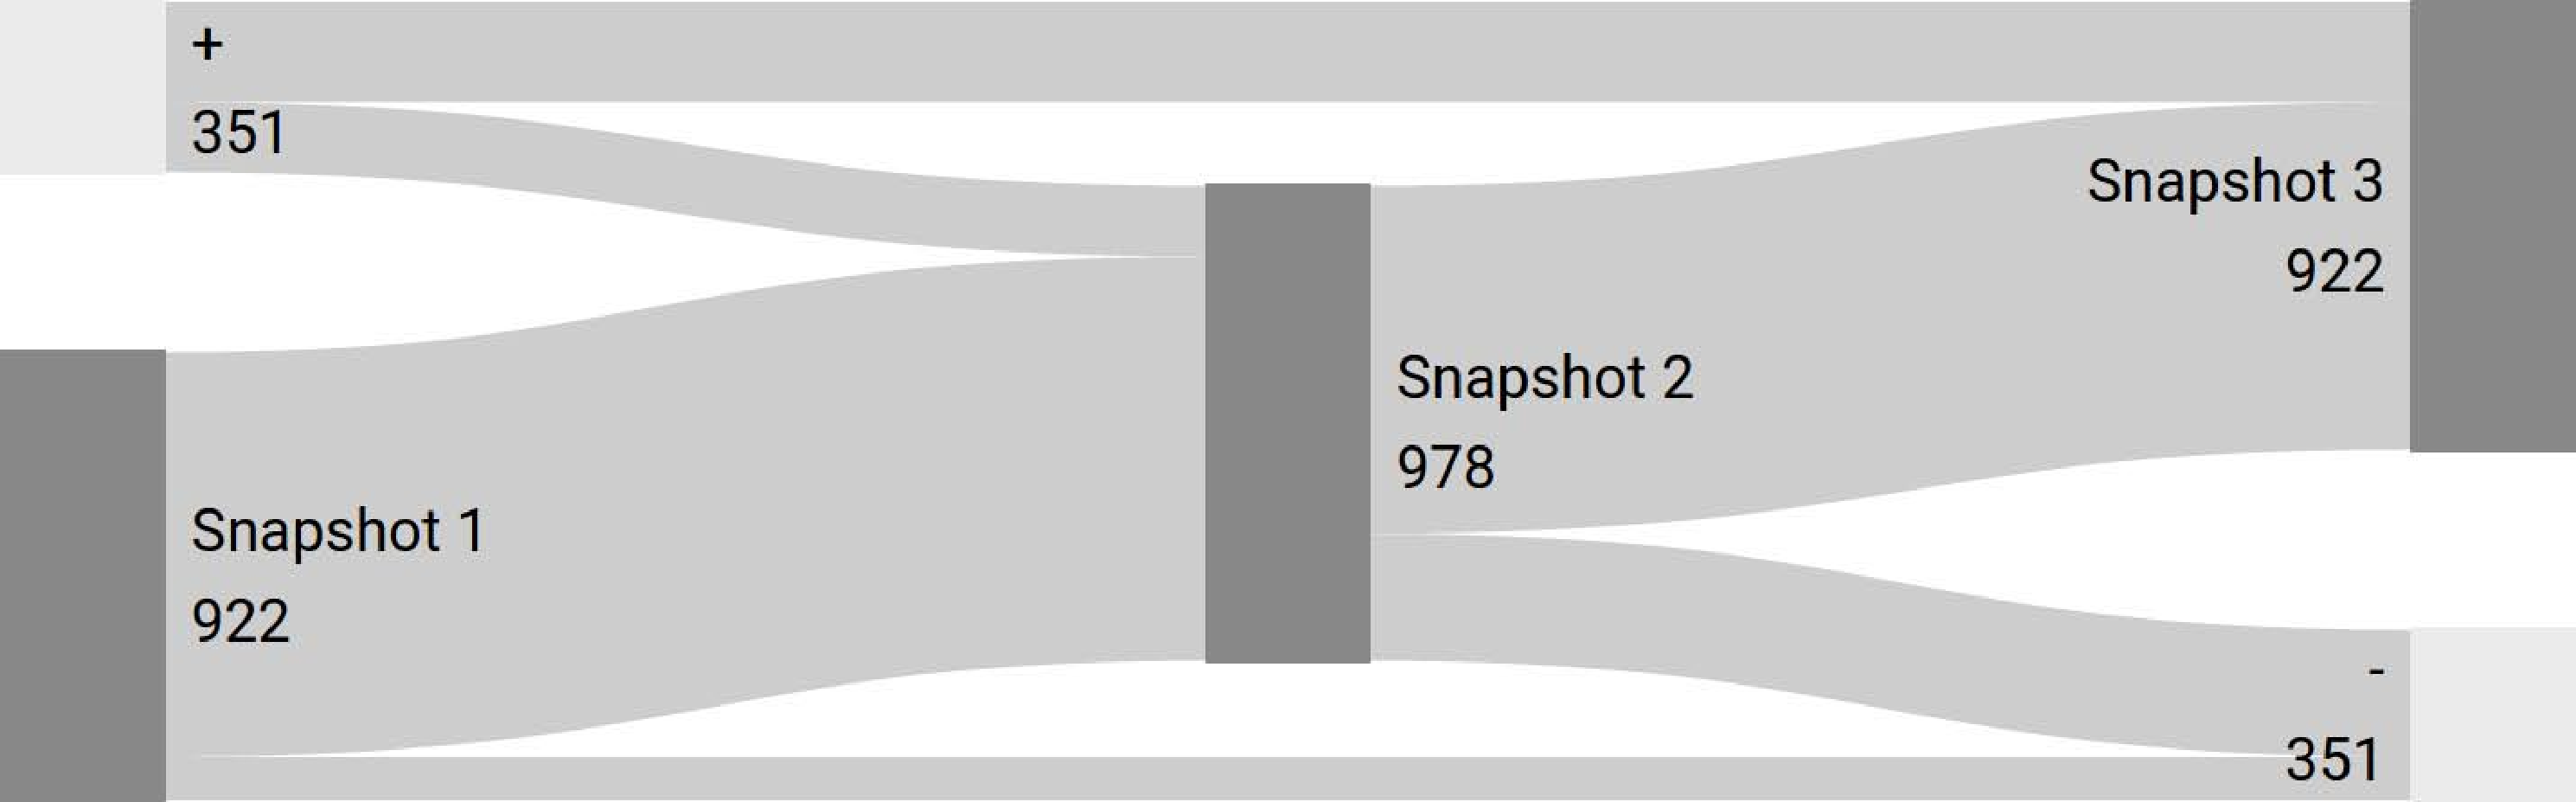
\includegraphics[width=.8\textwidth]{Figures/network_matching}
	\caption[Number of bees per snapshot]{\textbf{Number of bees per snapshot} This figure show the amount of bees for each snapshot and the proportion of intersecting bees between snapshots.}
	\label{fig:network-matching}
\end{figure}

Each snapshot consists of one large component.
Table~\ref{tab:stats} summarizes basic network properties.
For all, the density $D$ is over 50\%.
The diameter $\langle d_{\texttt{max}} \rangle$ is three and the average shortest path length $\langle d \rangle$ is below two.
The global clustering coefficient $C_\Delta$ of all snapshots is higher than compared to an Erdös-Renyi random graph, averaged over 100 runs using the same number of nodes and edges.
The high clustering coefficient and the small diameter suggest a small-world network type.
On average, each bee is connected to at least 50\% of all other bees in the network.

Figure~\ref{fig:fVSd} shows a positive correlation between the frequency of interactions and the total duration of interactions (averaged).
The frequency of interactions is used as weight of edges.
The edge weight distribution is shown in figure~\ref{fig:edgeWdist}.
Most edges have a low weight, only a few edges have a high weight.
It seems that bees do not prefer individuals bees for interaction.

\begin{table}[htbp]
\small
\centering
\caption[Global network properties]{\textbf{Global network properties} $N$ number of nodes, $L$ number of links, $D$ diameter, $\langle d_{\texttt{max}} \rangle$ average path length, $\langle d \rangle$ diameter, $C_\Delta$ global clustering coefficient, $\langle k \rangle$ average degree and $\langle s \rangle$ represents the average strength, as introduced in section~\ref{sec:definitions}.}
\label{tab:stats}
\vspace*{5mm}
\begin{tabular}{rccccccccc}
\toprule
{} &  $N$ &   $L$ &  $D$ &  $\langle d_{\texttt{max}} \rangle$ &  $\langle d \rangle$ &   $C_\Delta$ & $\langle k \rangle$ &  $\langle s \rangle$ \\
\midrule
Snapshot 1 & 922 & 291179 & 0.69 & 3 & 1.32 &  0.79 & 631.62 & 5680.17 \\
Random 1  & 922 & 291179 & 0.69 & 2 & 1.31 &  0.69 & 631.62 & - \\ \midrule
Snapshot 2 & 978 & 256066 & 0.54 & 3 & 1.46 &  0.72 & 523.65 & 3977.94 \\
Random 2  & 978 & 256066 & 0.54 & 2 & 1.46 &  0.54 & 523.65 & - \\ \midrule
Snapshot 3 & 922 & 259421 & 0.61 & 3 & 1.39 &  0.75 & 562.74 & 4205.99 \\
Random 3  & 922 & 259421 & 0.61 & 2 & 1.39 &  0.61 & 562.74 & - \\
\bottomrule
\end{tabular}
\end{table}

\begin{figure}[htb]
	\centering
	\begin{subfigure}[b]{0.49\textwidth}
	\centering
	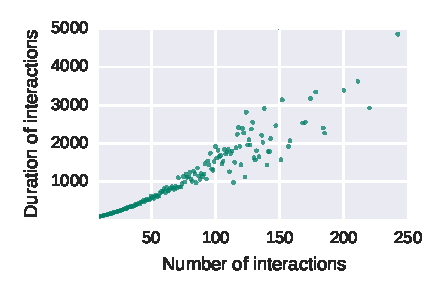
\includegraphics[width=1.0\textwidth]{Figures/n3-freqVSduration}
	\caption[Type of edge weights]{Type of edge weights}
	\label{fig:fVSd}
	\end{subfigure} 
	\begin{subfigure}[b]{0.49\textwidth}
	\centering
	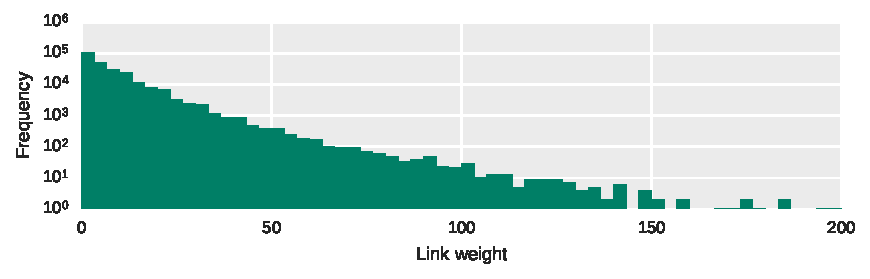
\includegraphics[width=1.0\textwidth]{Figures/n3-edgeWeightDist.pdf}
	\caption[Edge weight distribution]{Edge weight distribution}
	\label{fig:edgeWdist}
	\end{subfigure}
	\caption[Edge wights]{\textbf{Edge wights} }
	\label{fig:edges}
\end{figure}

\begin{figure}[htb]
	\centering
	\begin{subfigure}[b]{0.33\textwidth}
	\centering
	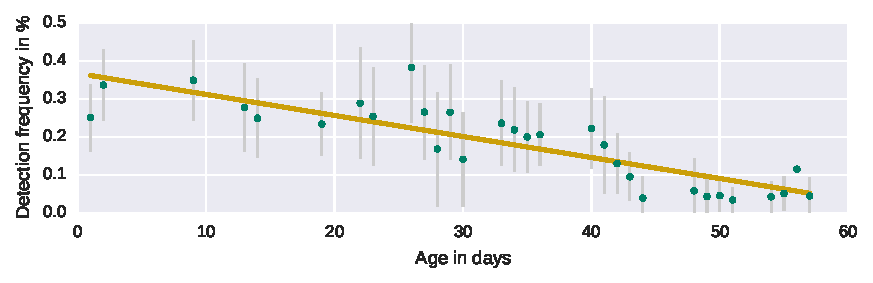
\includegraphics[width=1.0\textwidth]{Figures/n3_detFvsAge}
	\caption[]{}
	\label{fig:n3detfVSage}
	\end{subfigure} 
	\begin{subfigure}[b]{0.66\textwidth}
	\centering
	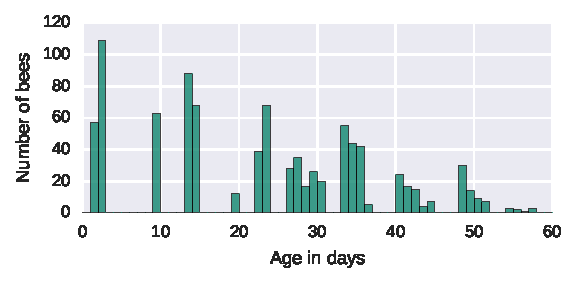
\includegraphics[width=1.0\textwidth]{Figures/n3_ages.pdf}
	\caption[]{}
	\label{fig:n3ageDist}
	\end{subfigure}
	\caption[X]{\textbf{X}}
	\label{fig:ageDetF}
\end{figure}


detection frequency distribution\\
age distribution\\
detection frequency vs age\\


\subsection{Degree, Strength and Local Clustering Coefficient}
type of network: no scale free\\
in relation to age and detection frequency\\
degree\\
strength\\
local clustering coefficient\\

\subsection{Betweenness and Closeness Centrality}
in relation to age and detection frequency\\
closeness\\
betweenness\\

\subsection{Communities}
table communities and members and age only for network 3\\
table KS nur für 3\\
plot age LE and WT\\
plot heatmap LE and heatmap WT\\